\section{Mixed-Precision HQR Factorization}
\label{sec:HQRf}

The HQR algorithm uses %a special type of linear transformations called 
Householder transformations to zero out elements below the diagonal of a matrix. 
We present this %the Householder transformation in the context of 
as zeroing out all but the first element of some vector, $\bb{x}\in\R^m$.

% TODO: this part could be expository, not a lemma. -GEOFF

\begin{lemma}
	Given vector $\bb{x}\in\R^{m}$, there exist Householder vector, $\bb{v}$, and Householder transformation matrix, $\bb{P}_{\bb{v}}$, such that $\bb{P}_{\bb{v}}$ zeros out $\bb{x}$ below the first element. 
	\begin{equation}
	\begin{alignedat}{3} 
	\sigma =& -\rm{sign}(\bb{x}_1)\|\bb{x}\|_2, &&\quad  \bb{v} = \bb{x} -\sigma \hat{e_1},\\
	\beta = & \frac{2}{\bb{v}^{\top}\bb{v}}=-\frac{1}{\sigma\bb{v}_1}, && \quad \bb{P}_{\bb{v}}=  \bb{I}_{m} - \beta \bb{v}\bb{v}^{\top}.
	\end{alignedat}
	\label{eqn:HH} 
	\end{equation}
	The transformed vector, $\bb{P_vx}$, has the same 2-norm as $\bb{x}$ since Householder transformations are orthogonal: $\bb{P}_{\bb{v}}\bb{x} = \sigma\hat{\bb{e}_1}$.
	In addition, $\bb{P}_{\bb{v}}$ is symmetric and orthogonal, $\bb{P}_{\bb{v}}=\bb{P}_{\bb{v}}^{\top}=\bb{P}_{\bb{v}}^{-1}$, and therefore, $\bb{P}_{\bb{v}}^2=\bb{I}$.
	\label{lem:hhvec}
\end{lemma}

\subsection{HQR Factorization Algorithm}
\label{sec:HQRfA}
Given $\bb{A}\in\R^{m\times n}$ and Lemma \ref{lem:hhvec}, HQR is done by repeating the following processes until only an upper triangle matrix remains.
For $i = 1, 2, \cdots, n,$
\begin{enumerate}[Step 1)]
	\item Compute $\bb{v}$ and $\beta$ that zeros out the $i^{th}$ column of $\bb{A}$ beneath $a_{ii}$, and
	\item Apply $\bb{P}_{\bb{v}}$ to the bottom right partition, $\bb{A}[i:m, i:n]$.
\end{enumerate}
%%% until only an upper triangular matrix remains. 

Consider the following $4$-by-$3$ matrix example adapted from \cite{Higham2002}. 
Let $\bb{P}_i$ represent the $i^{th}$ Householder transformation of this algorithm. 
\[\bb{A} = \left[ \begin{array}{ccc}
\times & \times & \times \\
\times & \times & \times \\
\times & \times & \times \\
\times & \times & \times
\end{array}
\right]\xrightarrow{\text{apply $\bb{P}_1$ to $\bb{A}^{(0)}:=\bb{A}$}}\left[ \begin{array}{c|cc}
\times & \times & \times \\ \hline
0 & \times & \times \\
0 & \times & \times \\
0 & \times & \times
\end{array}
\right]
\xrightarrow{\text{apply $\bb{P}_2$ to ($\bb{A}^{(1)}:=\bb{P}_1\bb{A}$)}}\]
\[ \left[
\begin{array}{cc|c}
\times & \times & \times \\
0 & \times & \times \\ \hline
0 & 0 & \times \\
0 & 0 & \times 
\end{array} \right]
\xrightarrow{\text{apply $\bb{P}_3$ to ($\bb{A}^{(2)}:=\bb{P}_2\bb{P}_1\bb{A}$)}} \left[ \begin{array}{ccc}
\times & \times & \times \\
0 & \times & \times \\
0 & 0 & \times \\
0 & 0 & 0 
\end{array}\right] \] 
% TODO: make fit on one line by writing A^(0)=[blah], P_1 A = [blah], P_2 P_1 A = [blah], etc ?? 
Since the final matrix $ \bb{P}_3\bb{P}_2\bb{P}_1\bb{A}$ is upper-triangular, this result is the $\bb{R}$ factor of the QR decomposition.
Set $\bb{Q}^{\top}:=\bb{P}_3\bb{P}_2\bb{P}_1$. 
Then, we can formulate  $\bb{Q}$ as
$$
\bb{Q} = (\bb{P}_3\bb{P}_2\bb{P}_1)^{\top} = \bb{P}_1^{\top}\bb{P}_2^{\top}\bb{P}_3^{\top} = \bb{P}_1\bb{P}_2\bb{P}_3,
$$
where the last equality results from the symmetric property of $\bb{P}_i$'s. 
%In addition, this is orthogonal because $\bb{Q}^{\top}=\bb{P}_3\bb{P}_2\bb{P}_1 =  \bb{P}_3^{\top}\bb{P}_2^{\top}\bb{P}_1^{\top} =  \bb{P}_3^{-1}\bb{P}_2^{-1}\bb{P}_1^{-1}=(\bb{P}_1\bb{P}_2\bb{P}_3)^{-1}=\bb{Q}^{-1}$, where the third equality results from the orthogonal property of $\bb{P}_i$'s.

Returning to the general case, we have
\begin{equation}
\bb{Q}_{\text{full}} = \bb{P}_1 \cdots \bb{P}_n\quad \text{and} \quad \bb{R}_{\text{full}} = \bb{Q}^{\top}\bb{A} = \bb{P}_n\cdots \bb{P}_1\bb{A},
\end{equation}
for the orthogonal factor in a full QR factorization, and
\begin{equation}
\bb{Q}_{\text{thin}} = \bb{P}_1 \cdots \bb{P}_n\bb{I}_{m\times n}\quad \text{and} \quad \bb{R}_{\text{thin}} = \bb{I}_{m\times n}^{\top}\bb{Q}^{\top}\bb{A} = \bb{I}_{m\times n}^{\top}\bb{P}_n\cdots \bb{P}_1\bb{A}.
\end{equation}

\subsubsection{HQR Factorization Implementation}
\label{sssec:HQRfI}
The Householder transformation is implemented by a series of inner and outer products, since Householder matrices are rank-1 updates of the identity. 
This approach is much less costly than forming $\bb{P}_{\bb{v}}$, and then performing matrix-vector or matrix-matrix multiplications.
For some $\bb{P}_{\bb{v}}=\bb{I}-\beta \bb{v}\bb{v}^{\top}$, we result in the following computation:
\begin{equation}
\label{eqn:hqrIO}
\bb{P}_{\bb{v}} \bb{x} = (\bb{I}-\beta \bb{v}\bb{v}^{\top})\bb{x} = \bb{x} - (\beta \bb{v}^{\top}\bb{x})\bb{v}.
\end{equation}
The routine in Equation \ref{eqn:hqrIO} is used in forming $\bb{R}$  and $\bb{Q}$. 
Given a vector $\bb{x}\in\R^{m}$, Algorithm \ref{algo:hh_v2} calculates the Householder constant, $\beta$, and Householder vector, $\bb{v}$, that zero out $\bb{x}$ below the first element and also returns $\sigma$. 
Algorithm \ref{algo:hhQR} is the HQR algorithm where information necessary to build $\bb{Q}$ is returned instead of explicitly forming $\bb{Q}$; the Householder vector and constant at the $k^{th}$ step are stored as the $k^{th}$ column of matrix $\bb{V}\in\R^{m\times n}$ and the $k^{th}$ element of vector $\bm{\beta}\in\R^n$. 

Finally, the $\bb{Q}$ factor can be built using Algorithm \ref{algo:hh_mult}.
While this algorithm shows how to left multiply $\bb{Q}$ to any input matrix $\bb{B}$ given $\bb{V}$ and $\bm{\beta}$, putting in $\bb{B}\equiv I_{m\times n}$ will yield $\bb{Q}_{\text{thin}}$.

\begin{algorithm2e}[H]
	\DontPrintSemicolon % Some LaTeX compilers require you to use \dontprintsemicolon instead
	\KwIn{$\bb{x}\in\R^m$}
	\KwOut{$\bb{v}\in\R^m$, and $\sigma, \beta\in\R$ such that $(I-\beta \bb{v}\bb{v}^{\top})\bb{x} = \pm \|\bb{x}\|_2 \hat{e_1} = \sigma\hat{e_1}$ }
	\tcc{We choose the sign of sigma to avoid cancellation of $\bb{x}_1$ (As is the standard in LAPACK, LINPACK packages \cite{Higham2002}). This makes $\beta>0$.}
	$\bb{v}\gets \bb{x}$\\
	$\sigma \gets -\rm{sign}(\bb{x}_1)\|\bb{x}\|_2$\\
	$\bb{v}_1 \gets \bb{x}_1-\sigma$ \tcp*{This is referred to as $\bb{\tilde{v}}_1$ later on.} 
	$\beta \gets -\frac{\bb{v}_1}{\sigma}$\\
	$\bb{v} \gets \frac{1}{\bb{v}_1}\bb{v}$\\
	\Return $\beta$, $\bb{v}$, $\sigma$
	\caption{$\beta$, $\bb{v}$, $\sigma = {\tt hh\_vec}(\bb{x})$. Given a vector $\bb{x}\in\R^n$, return the Householder vector, $\bb{v}$; a Householder constant, $\beta$; and $\sigma$ such that $(I-\beta \bb{v}\bb{v}^{\top})\bb{x} =\sigma(\hat{e_1})$ and $\bb{v}_1=1$, (see \cite{LAPACK, Higham2002}).}
	\label{algo:hh_v2}
\end{algorithm2e}

	\begin{algorithm2e}
	\DontPrintSemicolon % Some LaTeX compilers require you to use \dontprintsemicolon instead
	\KwIn{$A\in\R^{m \times n}$ where $m \geq n$.}
	
	\KwOut{$\bb{V}$,$\bm{\beta}$, $\bb{R}$}
%	\tcc{$\bb{v}_i = V[i:m, i] \in \R^{m-(i-1)}$ and $\bb{B}_i = \bb{B}[i:m, i:d] \in \R^{(m-(i-1))\times(d-(i-1))}$.}
	$\bb{V}, \bm{\beta} \gets \bb{0}_{m\times n}, \bb{0}_m$ \\
	
	\For{$i=1 : n$}{
		$\bb{v}, \beta, \sigma \gets \mathrm{hh\_vec}(\bb{A}[i:\mathrm{end}, i])$\\	
		$\bb{V}[i:\mathrm{end},i]$, $\bm{\beta}_i$,  $\bb{A}[i,i] \gets \bb{v}, \beta, \sigma$\tcp*{Stores the Householder vectors and constants.}
		\tcc{The next two steps update $\bb{A}$.}
		$\bb{A}[i+1:\mathrm{end}, i]\gets \mathrm{zeros}(m-i)$\\
		$\bb{A}[i:\mathrm{end}, i+1:\mathrm{end}]\gets \bb{A}[i:\mathrm{end}, i+1:\mathrm{end}] - \beta \bb{v} \bb{v}^{\top}\bb{A}[i:\mathrm{end}, i+1:\mathrm{end}]$
		
	}
	\Return $\bb{V}$, $\bm{\beta}$, $\bb{A}[1:n, 1:n]$
%	\caption{$\bb{V}$, $\bm{\beta}$, $\bb{R}$ = ${\tt qr}(A)$. Given a matrix $A\in\R^{m\times n}$ where $m\geq n$, return matrix $\bb{V}\in\R^{m\times n}$, vector $\bm{\beta}\in\R^{n}$, and upper triangular matrix $\bb{R}$. An orthogonal matrix $\bb{Q}$ can be generated from $\bb{V}$ and $\bm{\beta}$, and $\bb{QR}=\bb{A}$.}
	
	\label{algo:hhQR}
	\end{algorithm2e}

	\begin{algorithm2e}
		\DontPrintSemicolon % Some LaTeX compilers require you to use \dontprintsemicolon instead
		\KwIn{$\bb{V}\in\R^{m \times n}$, $\bm{\beta}\in\R^{n}$ where $m \geq n$. $\bb{B} \in\R^{m\times d}$.  }
		
		\KwOut{$\bb{Q}\bb{B}$}
		\tcc{$\bb{v}_i = V[i:m, i] \in \R^{m-(i-1)}$ and $\bb{B}_i = \bb{B}[i:\mathrm{end}, i:\mathrm{end}] \in \R^{(m-(i-1))\times(d-(i-1))}$.}
		\For{$i=1 : n$}{
			$\bb{B}_i \gets \bb{B}_i - \bm{\beta}_i \bb{v}_i(\bb{v}_i^{\top}\bb{B}_i)$}
		\Return $\bb{B}$
		\caption{$\bb{Q}\bb{B}\gets {\tt hh\_mult}(V, \bb{B})$: Given a set of householder vectors $\{\bb{v}_i\}_{i=1}^n$ and their corresponding constants $\{\bm{\beta}_i\}_{i=1}^n$, compute $\bb{P}_1\cdots \bb{P}_n\bb{B}$, where $\bb{P}_i := \bb{I} - \bm{\beta}_i\bb{v}_i\bb{v}_i^{\top}$}
		\label{algo:hh_mult}
	\end{algorithm2e}

		
\subsubsection{Normalization of Householder Vectors}
\label{sssec:NormalizeHV}
Equation \ref{eqn:HH} gives a single Householder transformation matrix $\bb{P}_{\bb{v}'}$ for all $\bb{v}'$ in $\mathrm{Span}(\bb{v})$, which allows for many different ways of normalizing the Householder vectors as well as the choice of not normalizing them.
However, this equivalence ($\bb{P}_{\bb{v}}\equiv \bb{P}_{\bb{v'}}$ for all $\bb{v}' \in \mathrm{Span}(\bb{v})$)  is not guaranteed due to rounding errors when using floating point numbers and operations.
When using high precision floating point numbers such as double-precision floats, rounding errors that accumulate from the normalization of Householder vectors rarely and barely contribute to the overall stability of the HQR algorithm performed.
In contrast, lower precision floating point numbers with limited dynamic range may be more sensitive to the un/normalization choice.
For example, if we leave the Householder vectors unnormalized while using half-precision, it is possible to accumulate $\tt{Inf}$'s in inner products of ``large'' vectors.
As a result,  picking a normalization scheme for $\bb{v}$ is important in low-precision calculations.
Some methods and reasons for the normalization of $\bb{v}$ are as follows:

\begin{itemize}
	\item Set the first element of $\bb{v}$,  $\bb{v}_1$, as $1$ for efficient storage of many Householder vectors,
	\item Set the 2-norm of $\bb{v}$ to $\sqrt{2}$ to always have $\beta=1$, or
	\item Set the 2-norm of $\bb{v}$ to $1$ to prevent extremely large values, and to always have $\beta=2$.
\end{itemize}
LINPACK and its successor LAPACK are benchmark software libraries for performing numerical linear algebra \cite{LAPACK}. 
The LAPACK implementation of the HQR factorization uses  the first method of normalizing via setting $\bb{v}_1$ to $1$ and is shown in Algorithm \ref{algo:hh_v2}. %http://www.netlib.org/lapack/explore-html/df/dc5/group__variants_g_ecomputational_ga3766ea903391b5cf9008132f7440ec7b.html
The first normalizing method adds an extra rounding error to $\beta$ and $\bb{v}$ each, whereas the remaining methods incur no rounding error in forming $\beta$, since $1$ and $2$ can be represented exactly.

%The error analysis in the subsequent section assumes that there may exist errors in both $\beta$ and $\bb{v}$ to get the worse-case scenario and to be consistent with the LINPACK implementation. 


% where machine precision is approximately $10^{-3}$ and the largest number is $65,504$, a careful selection of the normalization may be necessary to acquire higher stability in the HQR algorithm.

\subsection{Rounding Error Analysis}
\label{sec:HQRre}
We present an error analysis for the HQR factorization where all inner products are performed with mixed-precision, and all other calculations are done in the storage precision, $w$.

Assumption~\ref{assump:mp} lays out the generalized mixed-precision inner product we will be using over and over again in the remainder of this paper.

\begin{assump}
	\label{assump:mp}
	Let $w$, $p$, and $s$ each represent floating point precisions for storage, product, and summation, where the varying precisions are defined by their unit round-off values denoted by $u_w$, $u_p$, and $u_s$, and we can assume $1\gg u_w \gg u_s$ and $u_p\in (0, u_w]$. 
	Within the inner product subroutine, products are done in precision $p$, summation is done in precision $s$, and the result stored in precision $w$.
	All operations other than inner products are done in the storage precision, $w$.
\end{assump}

\subsubsection{Error analysis for forming Householder Vector and Constant}
Calculating the Householder vector and constant is a major routine for the HQR factorization. 

\paragraph{Error analysis for $\bb{v}$}
In this section, we show how to bound the error when employing the mixed precision dot product procedure for Algorithm \ref{algo:hh_v2}.
We begin by extending the inner-product error shown in Lemmas~\ref{lem:ip_a} and \ref{lem:ip_b} to the 2-norm error. 
\par

\begin{lemma}[2-norm round-off error]
	\label{lem:2norm_a}
	Consider a mixed-precision scheme as is outlined in Assumption~\ref{assump:mp}.
	Let $\bb{x}\in \F_w^{m}$ be an arbitrary $n$-length vector stored in $w$ precision.
	The forward error bound for computing the 2-norm of $\bb{v}$ is
	\begin{equation}
	\fl(\|\bb{x}\|_2)= (1+\tth_w^{(d+z+1)})\|\bb{x}\|_2,
	\end{equation}
	where $|\tth_w^{(d+z+1)}|\leq \gamma_w^{(d+z+1)}|\bb{x}|$ for $z\in\{1,2\}$ and $d:=\lfloor\frac{(m-1)u_s}{u_w}\rfloor$.
\end{lemma} 
There is no error incurred in evaluating the sign of a number or flipping the sign. 
Therefore, the error bound for computing $\sigma = -\rm{sign}(\bb{x}_1)\|\bb{x}\|_2$ is exactly the same as that for the 2-norm, i.e.,
\begin{equation}
\label{eqn:sigma}
\fl(\sigma) = \hat{\sigma} = \rm{fl}(-\rm{sign}(\bb{x}_1)\|\bb{x}\|_2) = \sigma + \Delta \sigma,\quad |\Delta\sigma| \leq \gamma_w^{(d+z+1)}|\sigma|.
\end{equation}

Let $\bb{\tilde{v}}_1$ be the penultimate value $\bb{v}_1$ held ($\bb{\tilde{v}}_1 = \bb{x}_1-\sigma$).
We can now show the round-off error for $\bb{\tilde{v}}_1$ and $\bb{v}_i$, where $i=2 , \cdots, n$. 
Then the round-off errors for $\bb{\tilde{v}}_1$ and $\bb{v}_i$'s are
\begin{align*}
\fl(\bb{v}_1)&=\hat{\bb{v}_1} = \bb{\tilde{v}}_1 + \bb{\Delta \tilde{v}}_1, \\
&= \fl(\bb{x}_1-\hat{\sigma})= (1+\dd_w) (\sigma + \Delta\sigma) = (1+\tth_w^{(d+z+2)})\bb{\tilde{v}}_1,
\end{align*}
and
\begin{equation*}
\fl(\bb{v}_i)=\hat{\bb{v}_i} = \fl\left(\frac{\bb{x}_i}{\hat{\bb{v}_1}}\right) = (1+\dd_w)\frac{\bb{x}_i}{\bb{\tilde{v}}_1 + \bb{\Delta \tilde{v}}_1}=(1+\theta_w^{(1+2(d+z+2))})\bb{\tilde{v}}_i.
\end{equation*}
The above equalities (as opposed to inequalities) are permitted since $\tth$ values are allowed to be flexible within the corresponding $\gamma$ bounds.%, and we summarize the above results for the whole vector in Lemma~\ref{lem:HQRv}.

\paragraph{Error analysis for $\beta$}
Now we show the derivation of round-off error for the Householder constant, $\beta$:
\begin{align*}
\hat{\beta} = \fl\left(-\frac{\hat{\bb{v}_1}}{\hat{\sigma}}\right) &=-(1+\dd_w)\frac{\bb{\tilde{v}}_1+\bb{\Delta \tilde{v}}_1}{(\sigma + \Delta\sigma)} %%%\\
%%%&
= -(1+\tth_w^{(1)})\frac{ (1+\tth_w^{(d+z+2)})\bb{v}_1}{(1+\tth_w^{(d+z+1)})\sigma} %%%\\
%%%&
= (1+\tth_w^{(d+z+3+2(d+z+1))})\beta,\\
&= (1+\tth_w^{(3d+3z+5)})\beta,
\end{align*}
where $z=1$ or $z=2$, depending on which mixed-precision inner product procedure was used. 
These two results are formalized in Lemma~\ref{lem:HQRv} below.
\begin{lemma}
	\label{lem:HQRv}
	Given $\bb{x}\in\R^{m}$, consider the constructions of $\beta\in\R$ and $\bb{v}\in\R^{m}$ such that $\bb{P}_{\bb{v}}\bb{x}=\sigma\hat{e_1}$ (see Lemma~\ref{lem:hhvec}) by using Algorithm~\ref{algo:hh_v2}.
	Then the forward error of forming $\bb{v}$ and $\beta$ with the floating point arithmetic with the
	mixed-precision scheme outlined in Assumption~\ref{assump:mp} are
	\begin{equation*}
	\|\hat{\bb{v}}\|_2 = (1+\theta_w^{(1+2(d+z+2))})\|\bb{v}\|_2 \qquad \mbox{and} \qquad
	\hat{\beta} = (1+\tth_w^{(3d+3z+5)})\beta,
	\end{equation*}
	where $z\in\{1,2\}$ and $d=\lfloor\frac{(m-1)u_s}{u_w}\rfloor$.
\end{lemma}
%TODO: when \beta is 1 or \sqrt(2), is there any error for beta?   If not, comment regarding this...   -Geoff
%\sqrt{2} is NOT exact, but 1 is. -Minah
%TODO: present theorem from Higham, and make comparison at the very end of this section. 
%\paragraph{Comparison to uniform precision analysis:}
%In this paper, uniform precision refers to using the same precision for all floating point operations. 
%We compare the errors for $\hat{\beta}$ and $\hat{\bb{v}}$ computed via the mixed-precision inner products to the errors computed while everything was done in half-precision. 
%
%To simplify error analyses even further, we now introduce the $\tilde{\gamma}$ notation in Equation \ref{eqn:tildegamma}, which is introduced in Section 19.3 of \cite{Higham2002}.
%This notation allows us to keep track of only the leading order floating point operations. 
%For example, in the HQR factorization routine, computation of dot products is the most costly subroutine, as the number of FLOPs linearly depends on the number of rows, $m$, in the original matrix.
%It is sufficient 
%Without mixed-precision, the errors would be bounded by
%\begin{equation}
%\tilde{\gamma}^{(k)} := \frac{cku}{1-cku},
%\label{eqn:tildegamma}
%\end{equation}
%and $c$ is a small integer (c.f. Section 19.3 \cite{Higham2002}).
%%This new $\tilde{\gamma}$ notation is introduced in \cite{Higham2002} to further simplify error analyses by caring only about leading-order floating point operations. 
%Let us further assume that the storage precision ($u_{w}$) in the mixed-precision analysis is half-precision. 
%In other words, we can let $u\equiv u_w$, and directly compare $\tilde{\gamma_w}^{(m)}$ and $\gamma_w^{(3d+3z+5)}$.
%The integer $d$ depends on the length of the vector, $m$ and the precisions ($u_w$ and $u_s$), and likely is a small integer.
%For example, if storage is done in half-precision, and summation within the inner product is done in single-precision, then $d :=\lfloor\frac{m-1}{8192}\rfloor$.
%Since both $d$ and $z$ are usually small integers, the errors for $\hat{\beta}$ and $\hat{\bb{v}}$ with mixed-precision arithmetic can be approximated by $\gamma_w^{(3d+3z+5)} \approx \tilde{\gamma_w}^{(d+z+1)}$.
%This is an improvement from $\tilde{\gamma_w}^{(m)}$ as $$m \gg \lfloor\frac{m-1}{8192}\rfloor + z + 1.$$

\subsubsection{Applying a Single Householder Transformation}
A Householder transformation is applied through a series of inner and outer products, since Householder matrices are rank-1 updates of the identity. 

For some $\bb{P}_{\bb{v}}=I-\beta \bb{v}\bb{v}^{\top}$, we result in $\bb{P}_{\bb{v}} \bb{x} = (I-\beta \bb{v}\bb{v}^{\top})\bb{x} = \bb{x} - (\beta \bb{v}^{\top}\bb{x})\bb{v}$.
\paragraph{Applying $\bb{P}_{\bb{v}}$ to zero out the target column of a matrix}
Let $\bb{x}\in\R^{m}$ be the target column we wish to zero out beneath the first element.
Recall that we chose a specific $\bb{v}$ such that $\bb{P}_{\bb{v}}\bb{x} = \sigma \hat{e}_1$. 
As a result, the only error lies in the first element, $\sigma$, and that is shown in Equation \ref{eqn:sigma}.
Note that the normalization choice of $\bb{v}$ does not impact the Householder transformation matrix ($\bb{P}_{\bb{v}}$) nor its action on $\bb{x}$, $\bb{P}_{\bb{v}}\bb{x}$.

\paragraph{Applying $\bb{P}_{\bb{v}}$ to the remaining columns of the matrix}
Now, let $\bb{x}$ and $\bb{v}$ have no special relationship, as $\bb{v}$ was constructed given some preceding column.
Set $\bb{w}:= \beta \bb{v}^{\top}\bb{x}\bb{v}$.
Note that $\bb{x}$ is exact, whereas $\bb{v}$ and $\beta$ were still computed with floating point operations. 
The errors incurred from computing $\bb{v}$ and $\beta$ need to be included in addition to the new rounding errors accumulating from the action of applying $\bb{P}_{\bb{v}}$ to a column.

We show the error for forming $\fl\left(\bb{\hat{v}}^{\top}\bb{x}\right)$ first:
\begin{equation*}
\fl\left(\bb{\hat{v}}^{\top}\bb{x}\right) = (1+\tth_w^{(d+z)})(\bb{v}+\Delta\bb{v})^{\top}\bb{x}.
\end{equation*}
Where $\tth_w^{(d+z)}$ is incurred from the action of a dot product,
\begin{align*}
\fl\left(\bb{\hat{v}}^{\top}\bb{x}\right)&= (1+\tth_w^{(d+z)})(1+\tth_w^{(1+2(d+z+2))})\bb{v}^{\top}\bb{x},\\
&= (1+\tth_w^{(3d+3z+5)})\bb{v}^{\top}\bb{x}.
\end{align*}
Now we can form $\fl(\bb{w})$,
\begin{equation*}
\bb{\hat{w}} =(1+\tth_w^{(2)})(\beta+\Delta\beta)(1+\tth_w^{(3d+3z+5)})\bb{v}^{\top}\bb{x}\bb{w}.
\end{equation*}
Here, $\tth_w^{(2)}$ results from multiplying  $\hat{\beta}$ and $\bb{v}^{\top}\bb{x}$ to $\bb{w}$,
\begin{align*}
\bb{\hat{w}} &= (1+\tth_w^{(2)})(1+\tth_w^{(3d+3z+5)})\beta(1+\tth_w^{(3d+3z+5)})\bb{v}^{\top}\bb{x}\bb{w},\\
&= (1+\tth_w^{(6d+6z+12)})\bb{w}.
\end{align*}
% TODO - save some space in the previous 2 equations.

Finally, we can add in the vector subtraction operation and complete the rounding error analysis of applying a Householder transformation to any vector:
\begin{align}
\fl(\bb{P}_{\bb{v}}\bb{x}) & = \fl(\bb{x}-\bb{\hat{w}}) = (1+\dd_w)(1+\tth_w^{6d+6z+12)})\bb{w}, \\
&= (1+\tth_w^{(6d+6z+13)})\bb{P}_{\bb{v}}\bb{x},\\
&= (\bb{P_v} +\bb{\Delta P_v})\bb{x},\qquad \|\bb{\Delta P_v}\|_F \leq \gamma_w^{(6d+6z+13)}. \label{eqn:applyP}
\end{align}
Details behind the matrix norm error bound in Equation~\ref{eqn:applyP} are shown in \ref{Appendix:HQR}.
Constructing both $\bb{Q}$ and $\bb{R}$ relies on applying Householder transformations in the above two ways: 1) to zero out below the diagonal of a target column and 2) to update the bottom right submatrix. 
We now have the tools to formulate the forward error bound on $\hat{\bb{Q}}$ and $\hat{\bb{R}}$ calculated from the HQR factorization.
\subsubsection{HQR Factorization Forward Error Analysis}
%%% \begin{wrapfigure}{L}{0.5\textwidth}
%%% 	\begin{center}
%%%		%\centering
%%% 		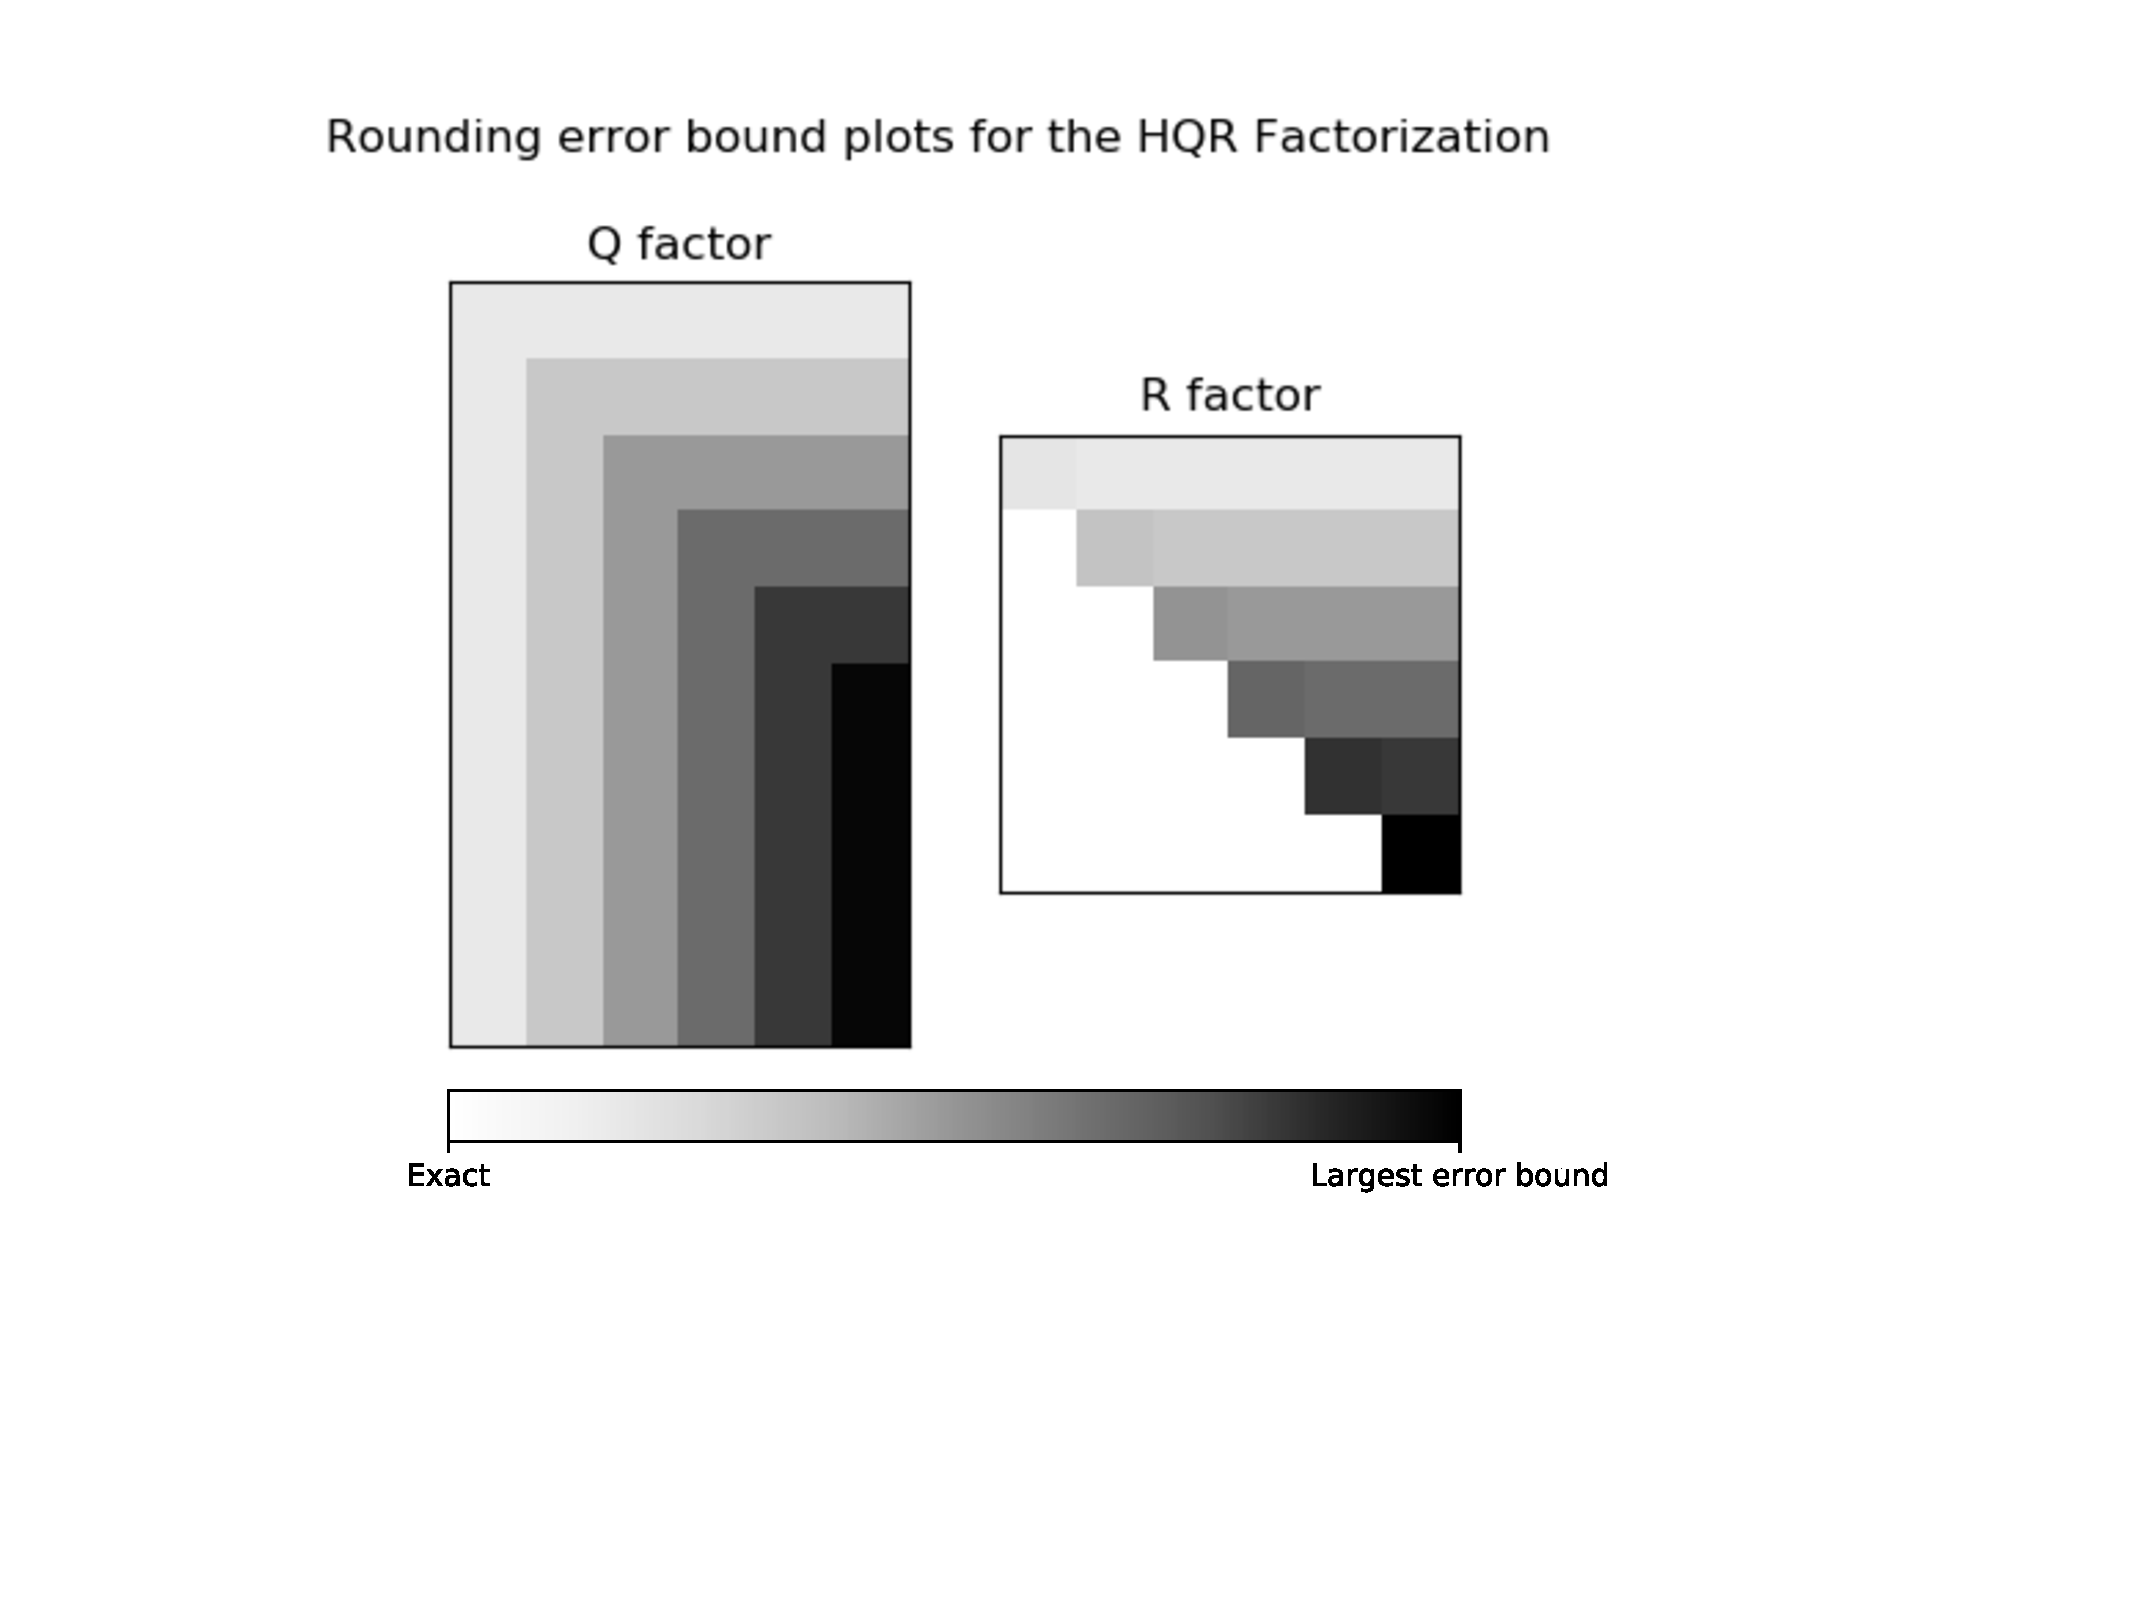
\includegraphics[width=0.5\textwidth]{./figures/figure2.pdf}
%%% 	\end{center}
%%% 	\caption{\label{fig:QRerr} Grayscale representation of distribution of rounding errors bounds for the HQR algorithm.}% Elements $\hat{\bb{R}}_{ij}=(1+\tth_w^{(r_{ij})})\bb{R}_{ij}$ and $\hat{\bb{Q}}_{ij}=(1+\tth_w^{(q_{ij})})\bb{Q}_{ij}$, where $r_{ij}$ and $q_{ij}$ are represented by grayscale.}	
%%% 	%\end{figure}
%%% \end{wrapfigure}

Consider a thin QR factorization where $\bb{A}\in\R^{m\times n}$ for $m\geq n$, we have $\bb{Q}\in\R^{m\times n}$ and $\bb{R}\in\R^{n\times n}$.
The pseudo-algorithm in Section \ref{sec:HQRf} shows that each succeeding Householder transformation is applied to a smaller lower right submatrix each time. \par
%For the $\bb{R}$ factor, everything beneath the diagonal is set to zero and therefore is exact, but all other elements incur rounding errors.
%These elements ($\hat{\bb{R}_{ii}}$ for $i\leq j$) go through $i-1$ Householder transformations designed to zero out $A^{(0)}[1:m, 1], A^{(1)}[2:m, 2], \cdots, A^{(i-2)}[i-1:m, i-1]$ that correspond to vectors of length $m, \cdots, m-(i-1)$.
%In addition, diagonal elements ($\hat{\bb{R}_{ii}}$) are then assigned $\hat{\sigma}$ from the process of zeroing out $A^{(i-1)}[i:m, i]$.
%Rounding errors for the $\bb{Q}$ factor can be formulated similarly. 
%Since the $i^{th}$ Householder transformation in building $\bb{Q}$ is performed on the $[i:m, i:n]$ lower-right submatrix, elements in $Q[i:m,i]$ and $Q[i,i:n]$ go through $i$ Householder transformations corresponding to vectors of sizes $m-(n-1), \cdots, m-(n-i)$ for $i = 1, \cdots, n$.

%Consequently, rounding error bounds for each element of $\bb{R}$ and $\bb{Q}$ can be specifically computed by its location within the matrices, as is displayed in Figure~\ref{fig:QRerr} for a $10$-by-$6$ example.
Instead of continuing with a componentwise analysis of how accumulated rounding errors are distributed by HQR, we transition into normwise error analyses.
To do this, we use the analysis from the preceding section (summarized in Equation~\ref{eqn:applyP}) to implicitly form the matrix norm error of the Householder transformation matrix, $\bb{P_v}$.
Then, we use the result of Lemma 3.7 in \cite{Higham2002} to get a normwise bound on the perturbation effect of multiple matrix multiplications.
This result is summarized in Theorem~\ref{thm:feHQR}, and the proof is detailed extensively in \ref{Appendix:HQR}.
%Then, we use the number of Householder transformations a column of $\bb{A}$ goes through to be transformed into a column of $\bb{R}$, and implicitly find the matrix norm error of the $\bb{Q}^{\top}$ that is formed in the process.
%Note that columnwise norms are easily converted to matrix norms (c.f. Lemma 6.6 in\cite{Higham2002}). 

\begin{theorem}
	\label{thm:feHQR}
	Let $\bb{A}\in\R^{m\times n}$ with $m\geq n$ have full rank, $n$. 
	Let $\hat{\bb{Q}}\in\R^{m\times n}$ and $\hat{\bb{R}}\in\R^{n\times n}$ be the thin QR factors of $\bb{A}$ obtained via the HQR algorithm with a mixed-precision scheme as is outlined in Assumption~\ref{assump:mp}.
	Let $d=\lfloor\frac{(m-1) u_s}{u_w}\rfloor$, and $z=1$ or $z=2$. 
	Then we have normwise forward error bounds
	\begin{align}
	\hat{\bb{R}} &= \bb{R} + \bb{\Delta R} = \hat{\bb{P}}_n\cdots\hat{\bb{P}}_1 \bb{A},\\
	\hat{\bb{Q}} &= \bb{Q} + \bb{\Delta Q} = \hat{\bb{P}}_1\cdots\hat{\bb{P}}_n \bb{I},
	\end{align}
	where
	\begin{equation}
	  \|\bb{\Delta Q}\|_F \leq n^{3/2} \tilde{\gamma}_w^{(6d+6z+13)},
	\end{equation}
	and for column $j$ in $\{1, \cdots, n\}$,
	\begin{equation}
	\|\bb{\Delta R}[:,j]\|_2 \leq j\tilde{\gamma}_w^{(6d+6z+13)}\|\bb{A}[:,j]\|_2.
	\end{equation}
	We also form a backward error.
	Let $\bb{A}+\bb{\Delta A} = \hat{\bb{Q}}\hat{\bb{R}}$, where $\hat{\bb{Q}}$ and $\hat{\bb{R}}$ are obtained via Algorithm~\ref{algo:hhQR}.
	Then,
	\begin{equation}
	\|\bb{\Delta A}\|_F \leq n^{3/2}\tilde{\gamma}_w^{(6d+6z+13)}\|\bb{A}\|_F.
	\end{equation}
\end{theorem}

\subsubsection{HQR Comparison to Uniform Precision Analysis}
\label{sec:mpupHQRcomparison}
%Contributions from the mixed-precision inner product scheme on the results from Theorem~\ref{thm:feHQR} are shown directly at the level of a single Householder transformation, as shown in Equation~\ref{eqn:applyP}.
The mixed-precision segments of the analysis behind Theorem~\ref{thm:feHQR} derive from the mixed-precision inner product scheme outlined in Assumption~\ref{assump:mp} and are propagated to form the error bounds for a single Householder transformation as is shown in Equation~\ref{eqn:applyP}.
All steps to form the error bounds in Theorem~\ref{thm:feHQR} from the error bound for a single Householder transformation (Equation~\ref{eqn:applyP}) directly follow the analyses in Section 19.3 of \cite{Higham2002}.
In these steps, we generalize the single Householder transformation error bound, 
\begin{equation}
\fl(\bb{P}_{\bb{v}}\bb{x})= (\bb{P}_{\bb{v}} + \bb{\Delta P_{v}})\bb{x},\qquad \|\bb{\Delta P_v}\|_F \leq \epsilon,\label{eqn:applyPgen}
\end{equation}
for some small quantity $0<\epsilon\ll 1$, and propagate it through the for-loop in Algorithm~\ref{algo:hhQR}. 
This process then results in forward error bound coefficients $n\epsilon$ or $n^{3/2}\epsilon$.
Since this $\epsilon$ value remains constant, the rounding error analysis for both mixed-precision and uniform-precision schemes are essentially the same with different values for $\epsilon$.
The uniform precision equivalent of Equation~\ref{eqn:applyP} is shown in Equation~\ref{eqn:applyPup},
\begin{equation}
\fl(\bb{P}_{\bb{v}}\bb{x})= (\bb{P}_{\bb{v}} + \bb{\Delta P_{v}})\bb{x},\qquad \|\bb{\Delta P_v}\|_F \leq \tilde{\gamma}^{(m)},
\label{eqn:applyPup}
\end{equation}
which is derived in detail in \cite{Higham2002}.
Therefore, we only need to compare $\gamma^{(6d+6z+13)}$ against $\gamma^{(cm)}$, where $c$ is a small integer. 
Although $d$ relies on both $m$ and the precisions $w$ and $s$, we can generally assume that $cm\gg (6d+6z+13)$ in most mixed-precision settings.
%, where $c$ is a small integer constant. 
Therefore, the new bounds in Theorem~\ref{thm:feHQR} are much tighter than the existing ones and more accurately describe the kind of rounding error accumulated in mixed-precision computational settings.
%up to the level of a single Householder transformation as is shown in Equation~\ref{eqn:applyP}.
%
%All steps to form the error bounds in Theorem~\ref{thm:feHQR} from the error bound for a single Householder transformation (c.f. Equation~\ref{eqn:applyP}) result in coefficients of $\tilde{\gamma}_w^{(6d+6z+13)}$, and these steps directly follow the analyses in Section 19.3 of \cite{Higham2002}.
%In these steps, we generalize the single Householder transformation error bound, 
%\begin{equation}
%\fl(\bb{P}_{\bb{v}}\bb{x})= (\bb{P}_{\bb{v}} + \bb{\Delta P_{v}})\bb{x},\qquad \|\bb{\Delta P_v}\|_F \leq \epsilon,\label{eqn:applyPgen}
%\end{equation}
%for some small quantity $0<\epsilon\ll 1$, and propagate it through the for-loop in Algorithm~\ref{algo:hhQR}. 
%Since this $\epsilon$ value remains constant, the rounding error analysis for both mixed-precision and uniform-precision schemes are essentially the same with different values for $\epsilon$.
%Therefore, we only need to compare $\gamma^{(6d+6z+13)}$ against $\tilde{\gamma}^{(m)}$. 
%Although $d$ relies on both $m$ and the precisions $w$ and $s$, we can generally assume that $m\gg (6d+6z+13)$ in most mixed-precision settings. 
%Therefore, new bounds in Theorem~\ref{thm:feHQR} are much tighter than the existing ones, and more accurately describe the kind of rounding error accumulated in mixed-precision computational settings.